\documentclass[answers]{exam}

\usepackage[dvipsnames]{xcolor}
\usepackage{amsmath}
\usepackage{amsfonts}
\usepackage{amsthm}
\usepackage{microtype}
\usepackage{siunitx}
\DeclareSIUnit\year{yr}
\usepackage{pgfplots}
\usepackage{graphicx}
\usepackage{sidecap}
\sidecaptionvpos{figure}{c}
\usepackage{float}
\usepackage{gensymb}
\usepackage{tkz-euclide}
\usetkzobj{all}
\usepackage{commath}
\usepackage{steinmetz}

\newtheorem*{thm}{Theorem}

% russian integral
\usepackage{scalerel}
\DeclareMathOperator*{\rint}{\scalerel*{\rotatebox{17}{$\!\int\!$}}{\int}}

% \qformat{Question \thequestion: \thequestiontitle\hfill}

\begin{document}

\section*{NCEA Level 3 Trigonometry (exercise set)\\4. Identity Fishing}
\paragraph{Goal} To practice proving additional identities relating the trigonometric functions.

\begin{questions}
  \question Prove the following identites true for all angles $ x $.
    \begin{parts}
      \part $\displaystyle \sec 2x = \frac{\sec^2 x}{2 - \sec^2 x} $
      \part $\displaystyle \cos x + \sin x = \frac{\cos 2x}{\cos x - \sin x} $
    \end{parts}
  \question Write an expression for $ \cos 4x $ in terms of only $ \cos x $ (and powers and multiples of $ \cos x $).
  \question Fix two numbers $ 0 < \alpha < \pi/2 $ and $ 0 < \beta < \pi/2 $. Consider the following diagram.
            \begin{center}
              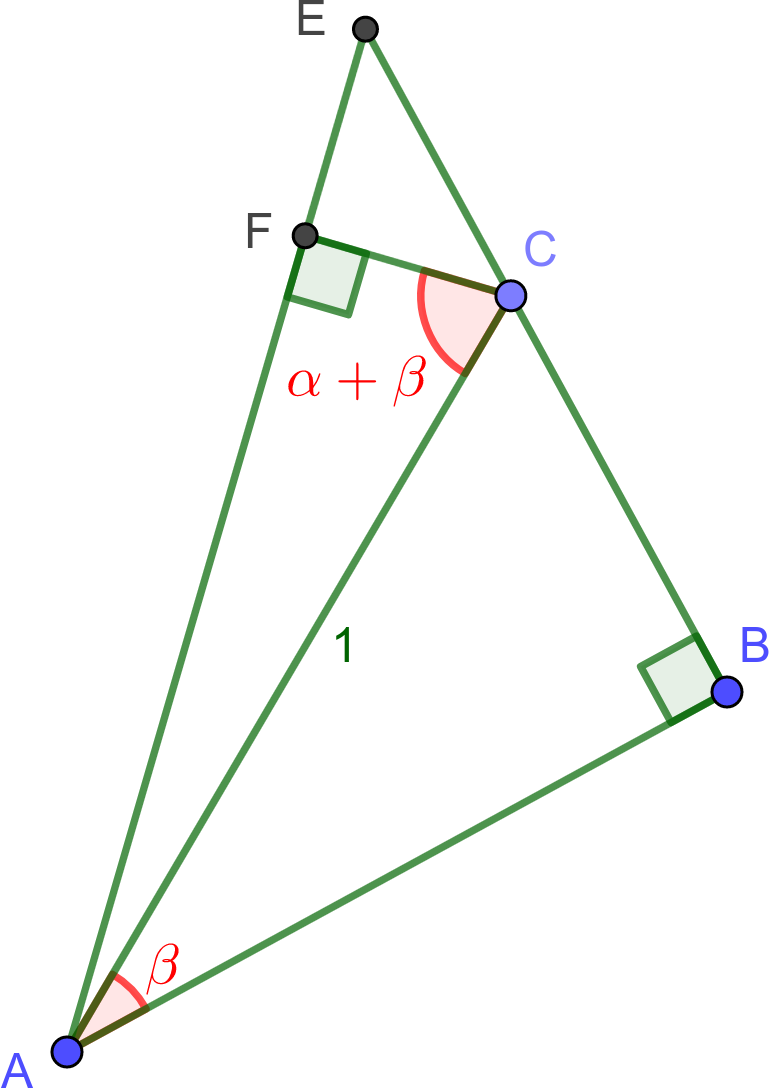
\includegraphics[width=0.3\textwidth]{cosinesum}
            \end{center}
            We have two right triangles, where $ ABC $ has an angle $ \beta $ and hypotenuse $ \abs{AC} = 1 $. From $ C $ we measure an angle $ \alpha + \beta $,
            and extend this line to meet a line from $ C $ at a right angle (so both interior angles at $ F $ are right). Hence $ \abs{AB} = \cos\beta $,
            $ \abs{BC} = \sin \beta $, and $ \abs{FC} = \cos(\alpha + \beta) $.
    \begin{parts}
      \part Show that the interior angle at $ E $ is $ \alpha $.
      \part Show that $ \abs{EC} = \frac{\cos (\alpha + \beta)}{\sin \alpha} $.
      \part Use (b) and the discussion below the diagram to show that
            \begin{displaymath}
              \frac{\abs{AB}}{\abs{BE}} = \frac{ \cos \beta }{\sin \beta + \frac{\cos (\alpha + \beta)}{\sin \alpha}}.
            \end{displaymath}
      \part Use (a) to show that $ \frac{\abs{AB}}{\abs{BE}} = \frac{\sin \alpha}{\cos \alpha} $.
      \part Prove that $ \cos(\alpha + \beta) = \cos \alpha \cos \beta - \sin \alpha \sin \beta $.
    \end{parts}
  \question Find all the points $ x $ such that $ \sin^2 x > \cos^2 x $.
  \question If $ a $, $ b $, $ c $, and $ d $ are the internal angles of a quadrilateral,
            show that
            \begin{displaymath}
              \cos (a+b+c) + \cos(b+c+d) + \cos(c+d+a) + \cos(d+a+b) = -4\cos \frac{a + b}{2} \cos \frac{a + c}{2} \cos \frac{a + d}{2}.
            \end{displaymath}
\end{questions}

\paragraph{Additional reading} Hobson, chapter IV, V.

\end{document}
